\section{时间隐通道检测方法}
\label{chap:backinfo:detect}

%本节主要介绍,现有的时间隐通道检测方法,主要包括哪些
时间隐通道的发展,催生了新的时间隐通道检测技术,适用性较好的是基于统计的时间隐通道检测方法。对于某些应用场景,基于标准差的检测方法和基于机器学习的检测方法,也是实际可行的。\nupcite{ARCHIBALD2014284}

\subsection{基于分布曲线的检测方法}
\label{chap:backinfo:detect:statistical}

%统计看CDF差异,主要评估了哪些参数
传输过程中的时间特征,是时间隐通道检测方法的检测目标,通常用于检测的对象为IPD。对于IPD来说,如果传输延迟恒定,则发送方观测到的IPD与接收方观测到的IPD是一致的。当网络噪声或者时间隐通道存在时,IPD取值出现偏离,监听方如果有标准的IPD分布参照,即可对比分布之间的最大偏离程度,从而判断是否存在风险。

\insertEquation{
    \begin{equation}
    \label{equ:2:ks}
		D_{KS}=sup_{x}|F_{1,n}(x)-G_{1,m}(x)|
    \end{equation}
    \begin{equation}
    \label{equ:2:ks-p}
        D_{KS,0.05}=1.358 \cdot \sqrt{\frac{n+m}{n \cdot m}}
    \end{equation}
}

\insertFigure{
	\begin{figure}
		\centering
        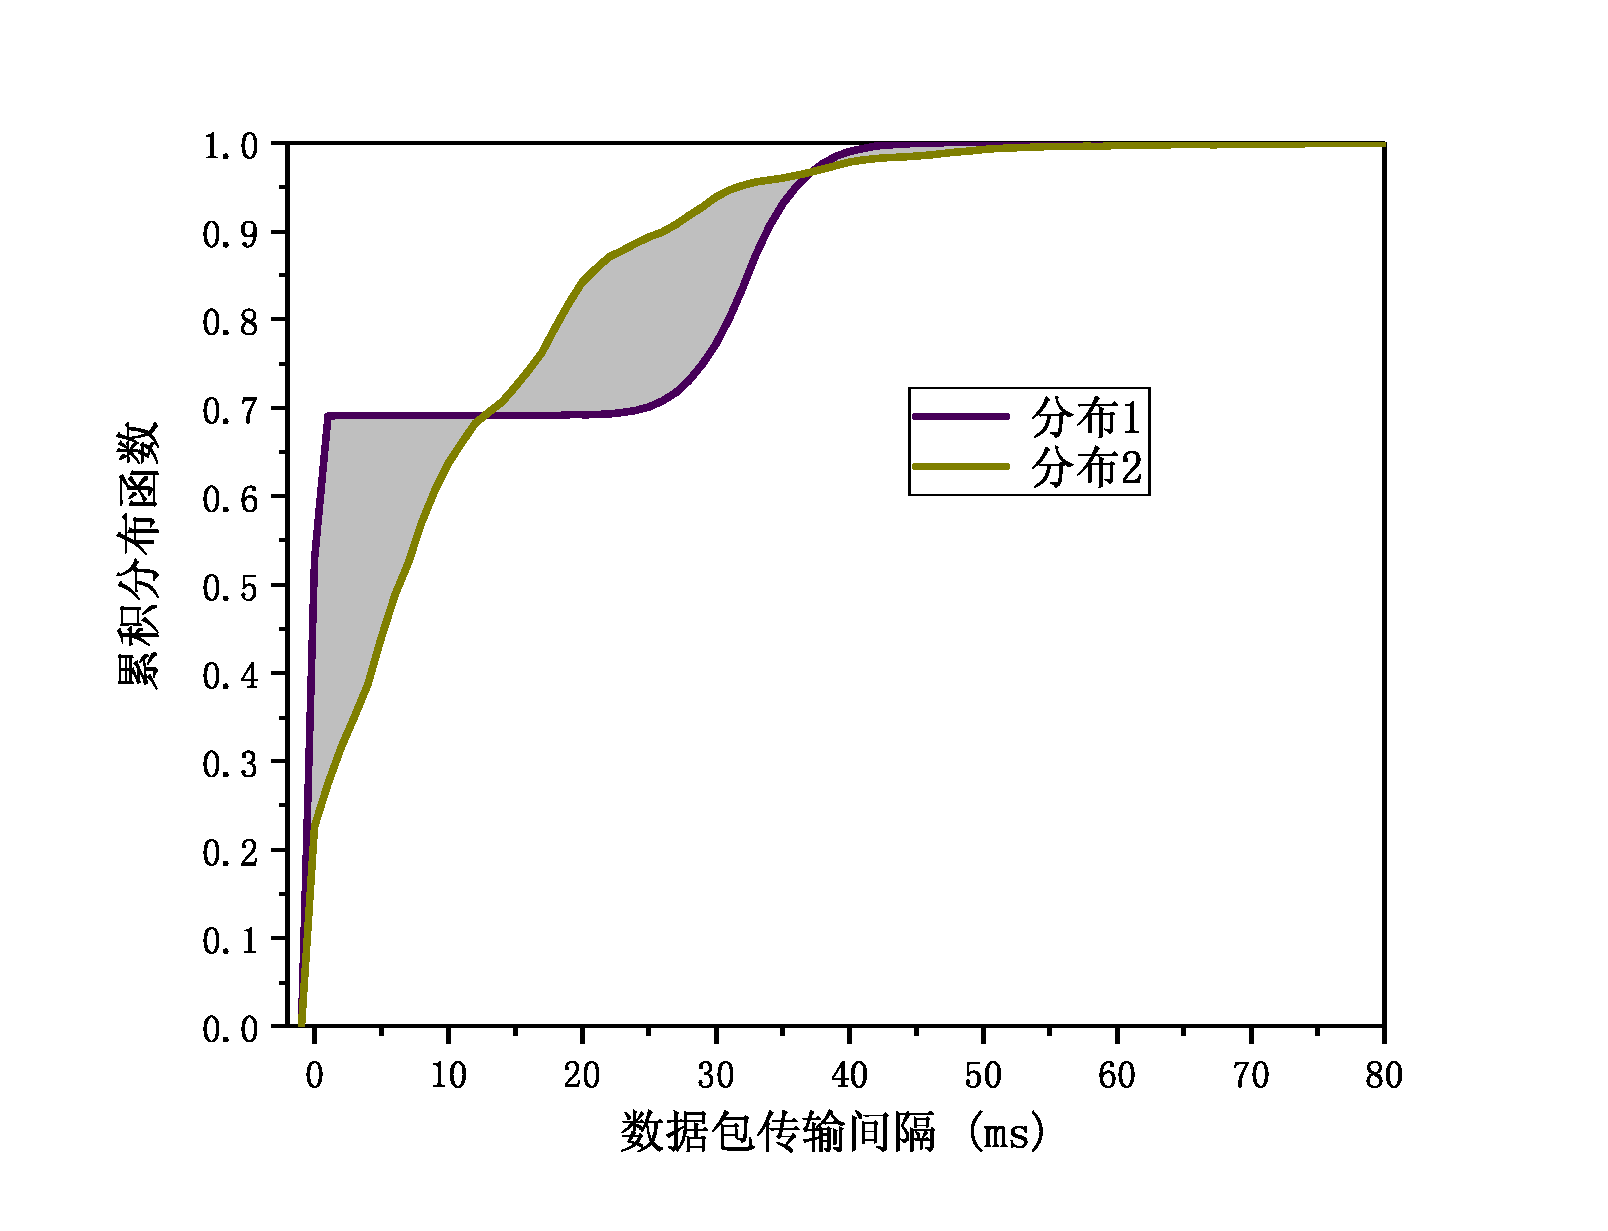
\includegraphics[width=0.9\textwidth]{chapters/chapter2/figures/ks-cdf.pdf}
        \caption{CDF曲线差异示意图}\label{fig:2:ks-cdf}
	\end{figure}
}

%如何根据差异,判断一致性
如图\nref{fig:2:ks-cdf},两种不同类型的CDF曲线,分别代表不同的IPD分布。通过公式(\nref{equ:2:ks}),计算分布曲线之间的差异的最大绝对值,得到分布曲线之间的直接差异。根据一致性假设理论,进行K-S测试的两个样本,在95\%一致概率的假设下,通过公式(\nref{equ:2:ks-p})计算置信值$D_{KS,0.05}$。当$D_{KS,0.05}>D_{KS}$时,即可判定$F_{1,n}$与$G_{1,m}$来自相同分布。

除了K-S测试外,常用的双样本测试方法还包括Welch’s t-test、Epps-Singleton (ES) test、Mann-Whitney rank test及Wilcoxon rank test等。各种测试方法在设计目标及适用对象方面,存在特定差异,实际应用场景需要进行辨别及选优。

\subsection{基于熵的检测方法}
\label{chap:backinfo:detect:entropy}

%计算熵,判断的对象是什么
数学统计中,Kullback–Leibler divergence又称相对熵,是一种判断两种概率质量函数差异的数学方法。在实际应用中,通过计算观测分布于已知分布之间熵值大小,判断两个分布之间的一致性。\nupcite{5590253,Gianvecchio:2007:DCT:1315245.1315284,Cabuk:2004:ICT:1030083.1030108,6296078}

\insertEquation{
    \begin{equation}
    \label{equ:2:kld}
		D_{KL}(F(x)||G(x))=\sum_{x=i}f(x) \cdot \log \frac{f(x)}{g(x)}
	\end{equation}
}

\insertTable{
	\begin{table}[]
        \centering
        \caption{IPD的概率质量函数示意表}
        \label{tab:2:pmf-dis}
        \begin{tabular*}{0.6\textwidth}{@{\extracolsep{\fill}}ccc}
        \toprule
        IPD & f(x) & g(x)\\ 
        \midrule
        0 & 0.52921 & 0.2265 \\ 
        1 & 0.16155 & 0.04827 \\ 
        2 & 0.00075 & 0.04231 \\ 
        3 & 0.00011 & 0.03467 \\ 
        4 & 0.00002 & 0.03603 \\ 
        5 & 0.00002 & 0.05287 \\ 
        \bottomrule
        \end{tabular*}
    \end{table}
}

如表\nref{tab:2:pmf-dis}所示,概率质量函数PMF(Probability Mass Function)对应的是不同IPD的统计概率,参照分布的概率函数为$g(x)$,样本分布的概率函数为$f(x)$。通过公式(\nref{equ:2:kld})计算$D_{KL}$,得到结果$0.278$,高于检测阈值$0.1$\nupcite{ZHANG201866},因此得出结论,样本与参照分布不一致,隐通道存在概率较高。

\subsection{基于机器学习的检测方法}
\label{chap:backinfo:detect:machine}

%机器学习的模型是怎样生成的
基于统计的时间隐通道检测方法,需要预先获取宿主信道的传输特征,并且检测方法针对的是特定构造方法。对于监听者来说,不仅需要获取时间隐通道的类型,还需要一定时间的观测数据才能得出判断。\nupcite{8875875,7087364}

%判定结果如何认定是否通过
基于SVM(Support Vector Machines)的检测方法,通过提取样本中的特征向量,用于训练SVM的分类器。识别过程中,提取检测样本中的指纹特征,通过训练过的SVM进行分类判断。用于训练的数据集,需要在已知时间隐通道的基础上,生成各种隐通道的传输特征,计算其K-S结果、KL散度及统计规律等特征。\nupcite{7087364}基于SVM的检测方法的优点,是在盲测情况下具有较好的效果,对于传输特征稳定的信道来说,具备良好的校测结果。

在VoLTE视频通话中,语音信道自身有明确的规律性,现有的检测方法均可实现准确判别。但对于视频信道来说,网络噪声存在不确定性,统计特征与通话场景及时间有关联,现有的检测方式无法有效应用。特别的,对于组合式时间隐通道,利用了多个信道中的时间特征,现有的方法在准确度方面面临挑战。